\documentclass[main.tex]{subfiles}
\clearpage
% Exercise 3
\section{Non-linear advection-diffusion equation}
Main focus of this section is going to be solving the viscous Burger's equation (VBE). As the title hints it contains parabolic and hyperbolic parts and is derived as a ``toy'' version from the family of non-linear hyperbolic equations with viscous terms (see 11.2 or E.15 in LV) in comparison to the well known Navier-Stokes equations.
\begin{alignat}{3}
  & \partial_t u(x,t) + \frac{1}{2} \partial_x \left( u(x,t)^2 \right) = \varepsilon \partial_{xx} u(x,t), \qquad && -1 < x < 1, && t > 0, \label{ex3:eq:vbe}\\
  & u(-1,t) = g_L(t), && && t > 0, \\ 
  & u(1,t) = g_R(t), && && t > 0, \\ 
  & u(x,0) = \eta(x), && -1 \leq x \leq 1.
\end{alignat}
The right hand side of equation \ref{ex3:eq:vbe} is called the viscous term (or heat conduction) and the term $\frac{1}{2} \partial_x \left( u(x,t)^2 \right)$ refers to the flux function. The handout mentions the fact that the solution $u$ is differentiable and the diffusion coefficient $\varepsilon$ is constant and greater than zero. Another important piece of information from the handout is the solution to the IBV problem for appropriate ICs and BCs given as:
\begin{equation}
    u(x,t) = - \tanh\left( \frac{x + 0.5 - t}{2\varepsilon} \right) + 1
\end{equation}
this function will be used to verify the numerical scheme that will proposed in the followin section.
% 3.1
\subsection{Stable numerical scheme}
Combining the numerical schemes from the first two sections gives rise to
\begin{equation}
    U_{j}^{n+1} = U_{j}^{n} \left(1 - \frac{\Delta t}{\Delta x}\left(U_{j}^{n} - U_{j-1}^{n}\right)\right) + \frac{\varepsilon \Delta t}{\Delta x^2}\left(U_{j+1}^{n} - 2 U_{j}^{n} + U_{j-1}^{n}\right)
\end{equation}
Von Neumann analysis was applied to this equation, however the term $g(\xi)$ could not be separated because of the multiplication in the $U^n_j (U^n_j - U^n_{j-1})$ term, so it was decided to test out the stability by choosing $\Delta t$ and $\Delta x$ by hand which unfortunately did not lead anywhere.
%% TODO: More about the first scheme that didn't work

Since the first scheme didn't yield much success, it was decided to find some similar scheme in the literature. C. Obertscheider's article on Burger's equations was chosen as a starting point and the scheme was modified to be:
%% TODO: Find a name for this scheme
\begin{equation}
    U^{n+1}_{j} = U^{n}_{j} + \frac{\varepsilon \Delta t}{\Delta x^2}\left( U^{n}_{j+1} - 2U^{n}_{j} + U^{n}_{j-1} \right) + \frac{1}{\Delta x}\left( f\left(U^{n}_{j+\frac{1}{2}}\right) - f\left(U^{n}_{j-\frac{1}{2}}\right) \right)
\end{equation}
where $f$ is the flux function $f(u) = \frac{1}{2}u^2$ and $f(U^{n}_{j\pm\frac{1}{2}})$ denotes the average of $f(U_j^n)$ and $f(U_{j\pm 1}^n)$.

%% TODO: Is it worth including von Neumann analysis if it leads nowhere?

% 3.2
\subsection{Matlab implementation and convergence}

The two schemes described were implemented in MATLAB although the second one seem to be more stable and produced better results. 

\lstinputlisting{../Ex3/BurgerSolver4.m}

\subsubsection*{Convergence}

Using the scheme given by equation 42 we compute the solution and calculated the local truncation error at the first point of the grid. Due to nonlinearities we were not able to obtain an expression for the stability of our methods. Hence, the grid was selected so that h and k satisfied the stability criteria of the FTCS solver found in the first exercise and the upwind method in the second exercise.

Figure shows a convergence plot where the two help lines reveal that with the correction the model order seems to be $\mathcal{O}(h^3 + k^2)$.

\begin{figure}[h]
    \centering
    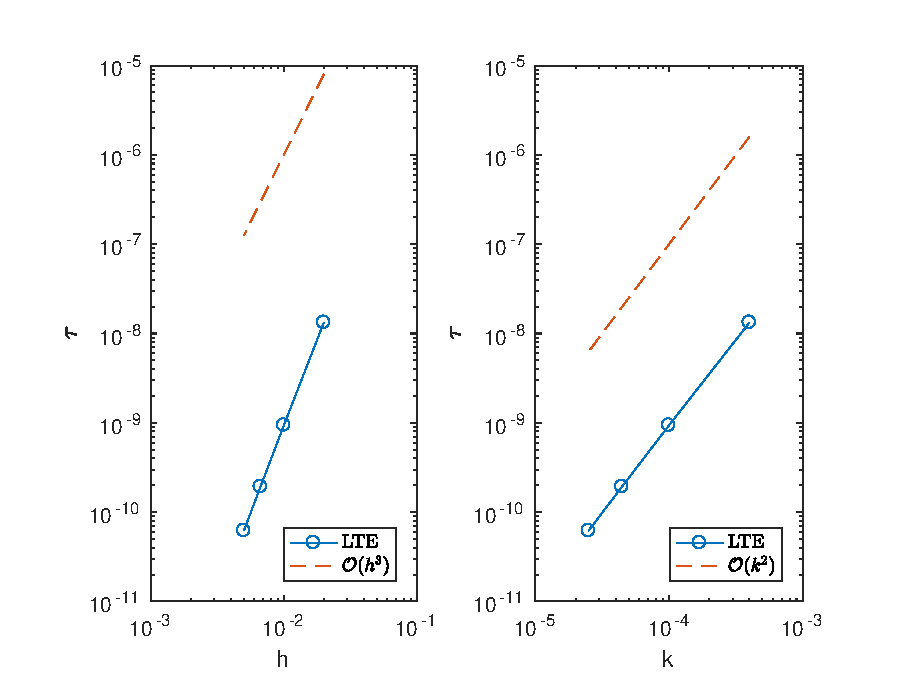
\includegraphics[width=\textwidth]{../Figures/3_3convergence}
    \caption{LTE for different values of $h$ and $k$}
\end{figure}

% 3.3
\subsection{Testing}
To demonstrate the implementation proposed in the previous section a problem is formulated as follows: $g_L(t) = g_R(t) = 0$ (homogenous BCs) and $\eta(x) = - \sin(\pi x)$. Solution will be found using an uniform grid and with $\varepsilon = \frac{1}{100 \pi}$. A figure will be presented demonstrating the solution at time $t_s = 1.6037/\pi$ along with value for $\partial_x u$ at $x=0$, which should be $-152.00516$ according to the handout. This value will be calculated as $\frac{u_c(\Delta x,t_s) - u_c(-\Delta x,t_s)}{2 \Delta x}$.

The derivative computed using the first scheme was not even close to the given value as can be seen in figure 9. This is due to the fact that the solver is unable to capture the stiff part. 

The second approach yielded a value of around -132 when setting h to 0.005 and $k = h^2$.

The nonuniform grid solver that will be presented in the last section, just using 35 points for x produced a value of -150.5 for the derivative, which seems to be the best out of all solvers we have tried.

\begin{figure}[h]
    \centering
    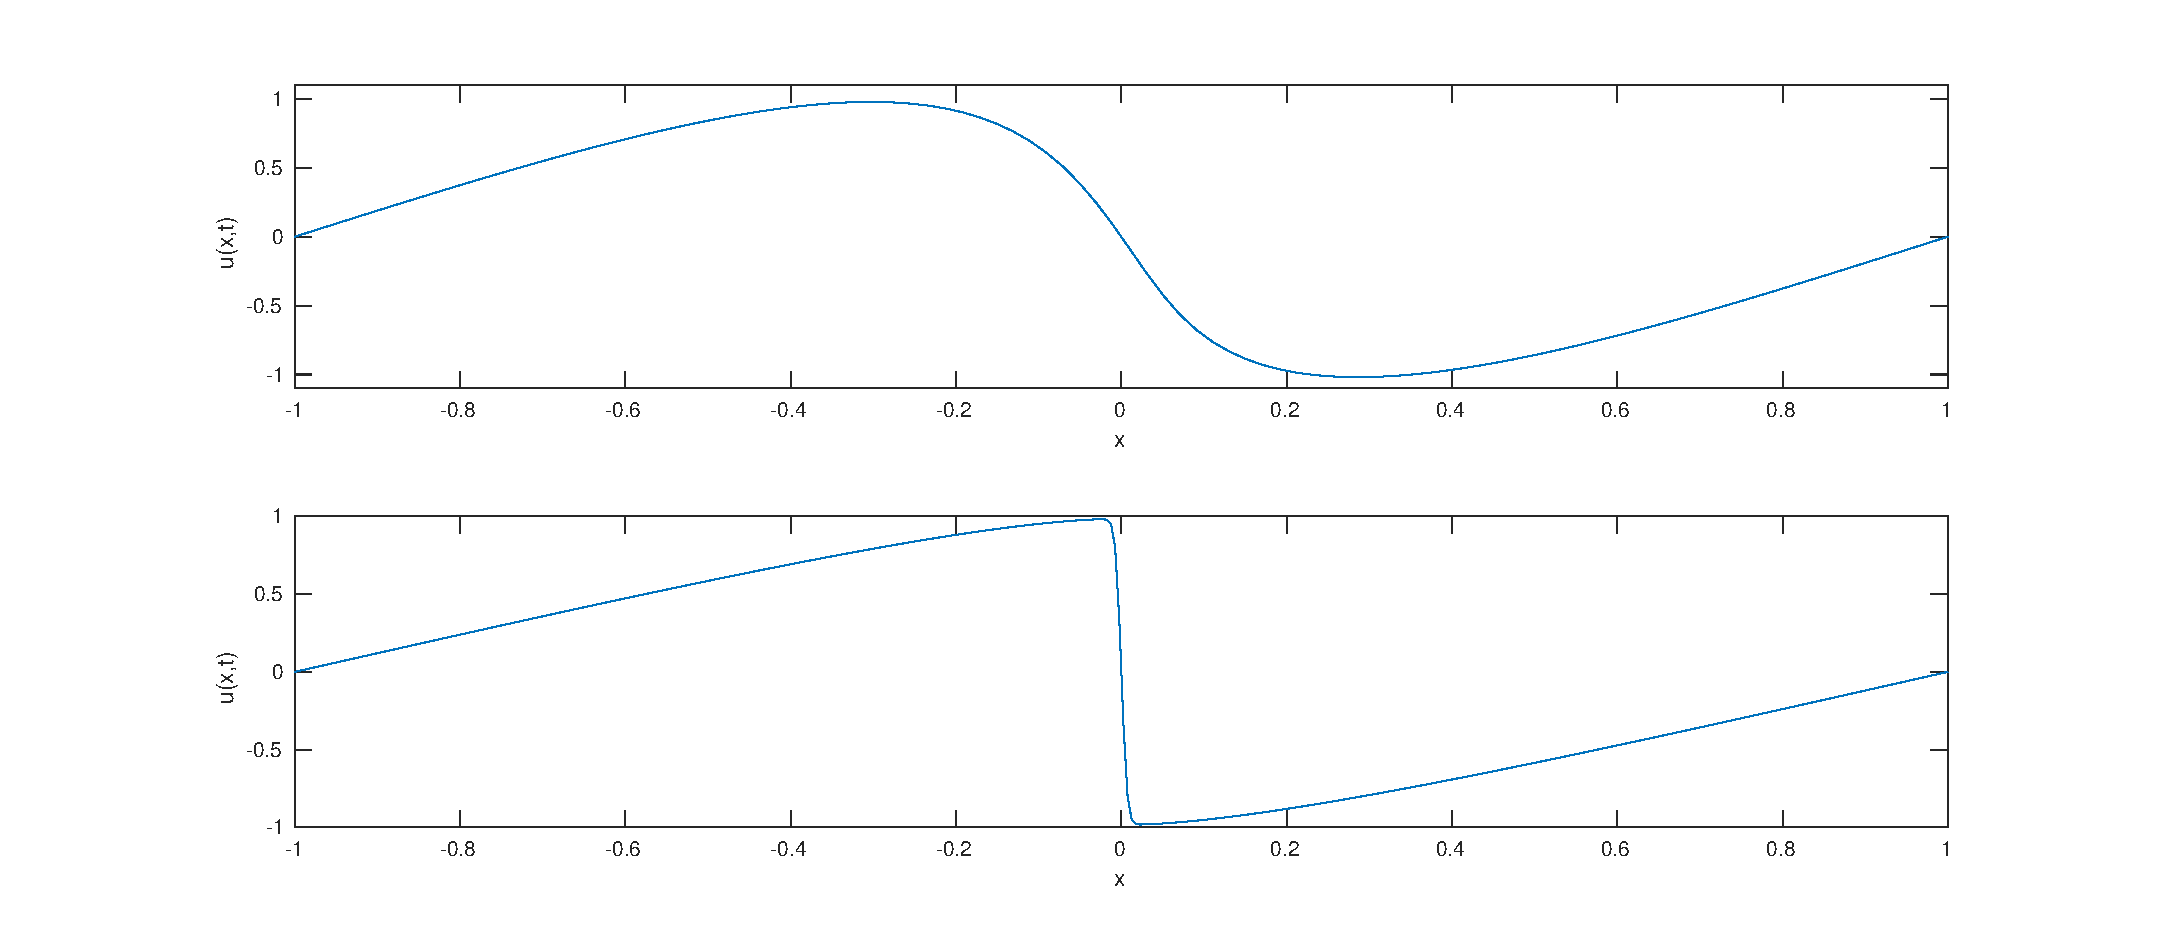
\includegraphics[width=\textwidth]{../Figures/sol3_3subplot}
    \caption{Solution at t=1.6037 using FTCS and upwind (top graph) FTCS and mid-point correction (bottom graph)}
\end{figure}

% 3.4
\subsection{Approaches to maintain accuracy}

As implementing a high-order accurate discretization method was too time consuming without leading to any results, it was decided to chose a non-uniform grid that captures the mid-points of the spatial domain in a finer manner.
\begin{figure}[h]
    \centering
    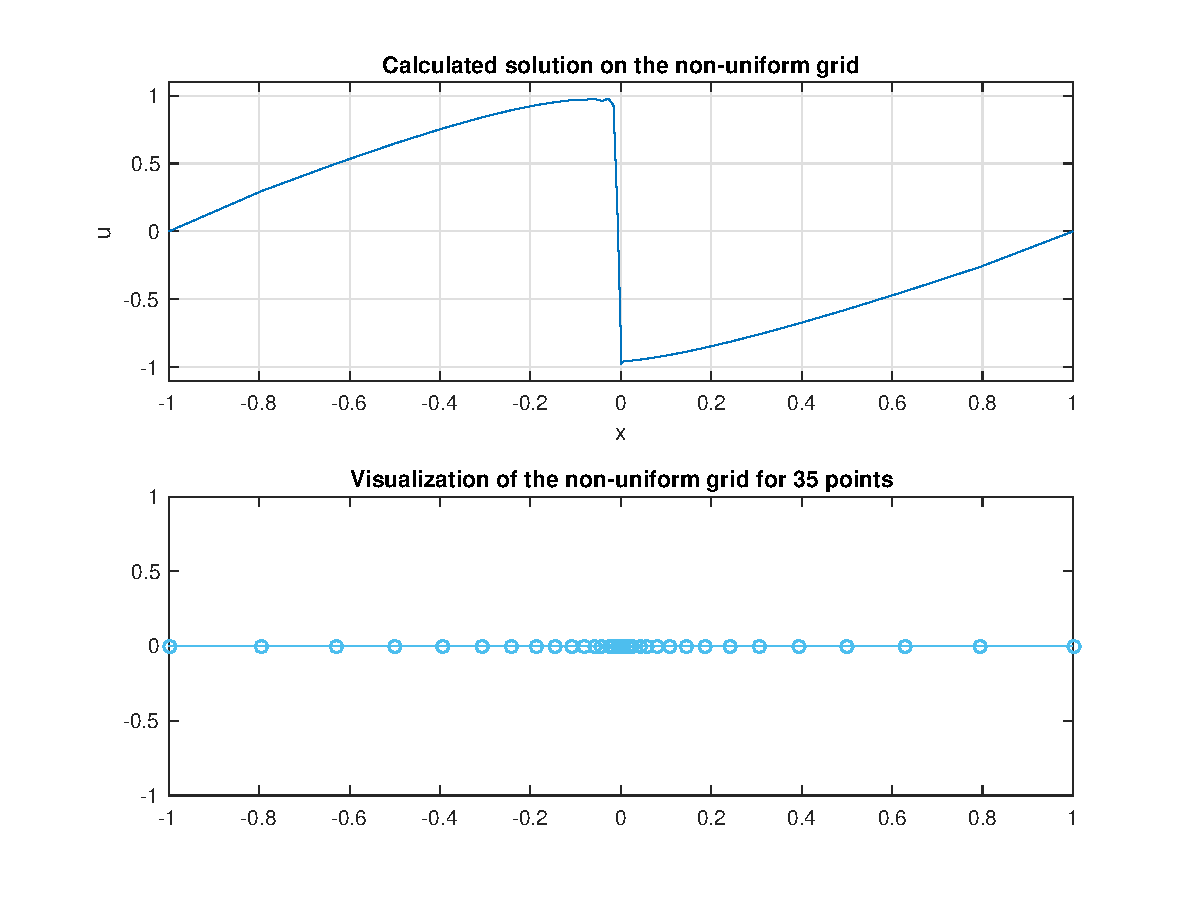
\includegraphics[height=3in]{../Figures/ex3_4_nonuniform}
    \caption{Non-uniform grid with 35 points concentrated mostly around 0 to try to capture the steep change of the slope}
\end{figure}
%% TODO: Include results for maintaining accuracy here















